\subsection{Обзор существующих аналогов клиент-серверного программного средства}
\label{sec:analysis:research:analogs}

На данный момент на рынке представлено достаточное количество мессенджеров, предоставляющих сквозное шифрование, но их всех объединяет один критический для бизнеса недостаток: отсутствие контроля. 
Пользовательские данные хранятся на серверах другой компании, нет доступа к инфраструктуре, код \gls{pp} часто является закрытым. Ниже будет рассмотрено несколько популярных аналогов и их подход к организации шифрования.

\subsubsection{}
\label{sec:analysis:research:analogs:telegram}

Одним из~самых популярных и~быстрорастущих мессенджеров современности является телеграм. 
Сервис разработан братьями Дуровыми и~частью бывшей комманды Вконтакте, криптография строится на~собственном протоколе MTProto.

На рисунке \ref{sec:analysis:research:analogs:telegram:ui} представлен список диалогов в~приложении Telegram и~пример секретного чата.

\begin{figure}[h]
  \centering
    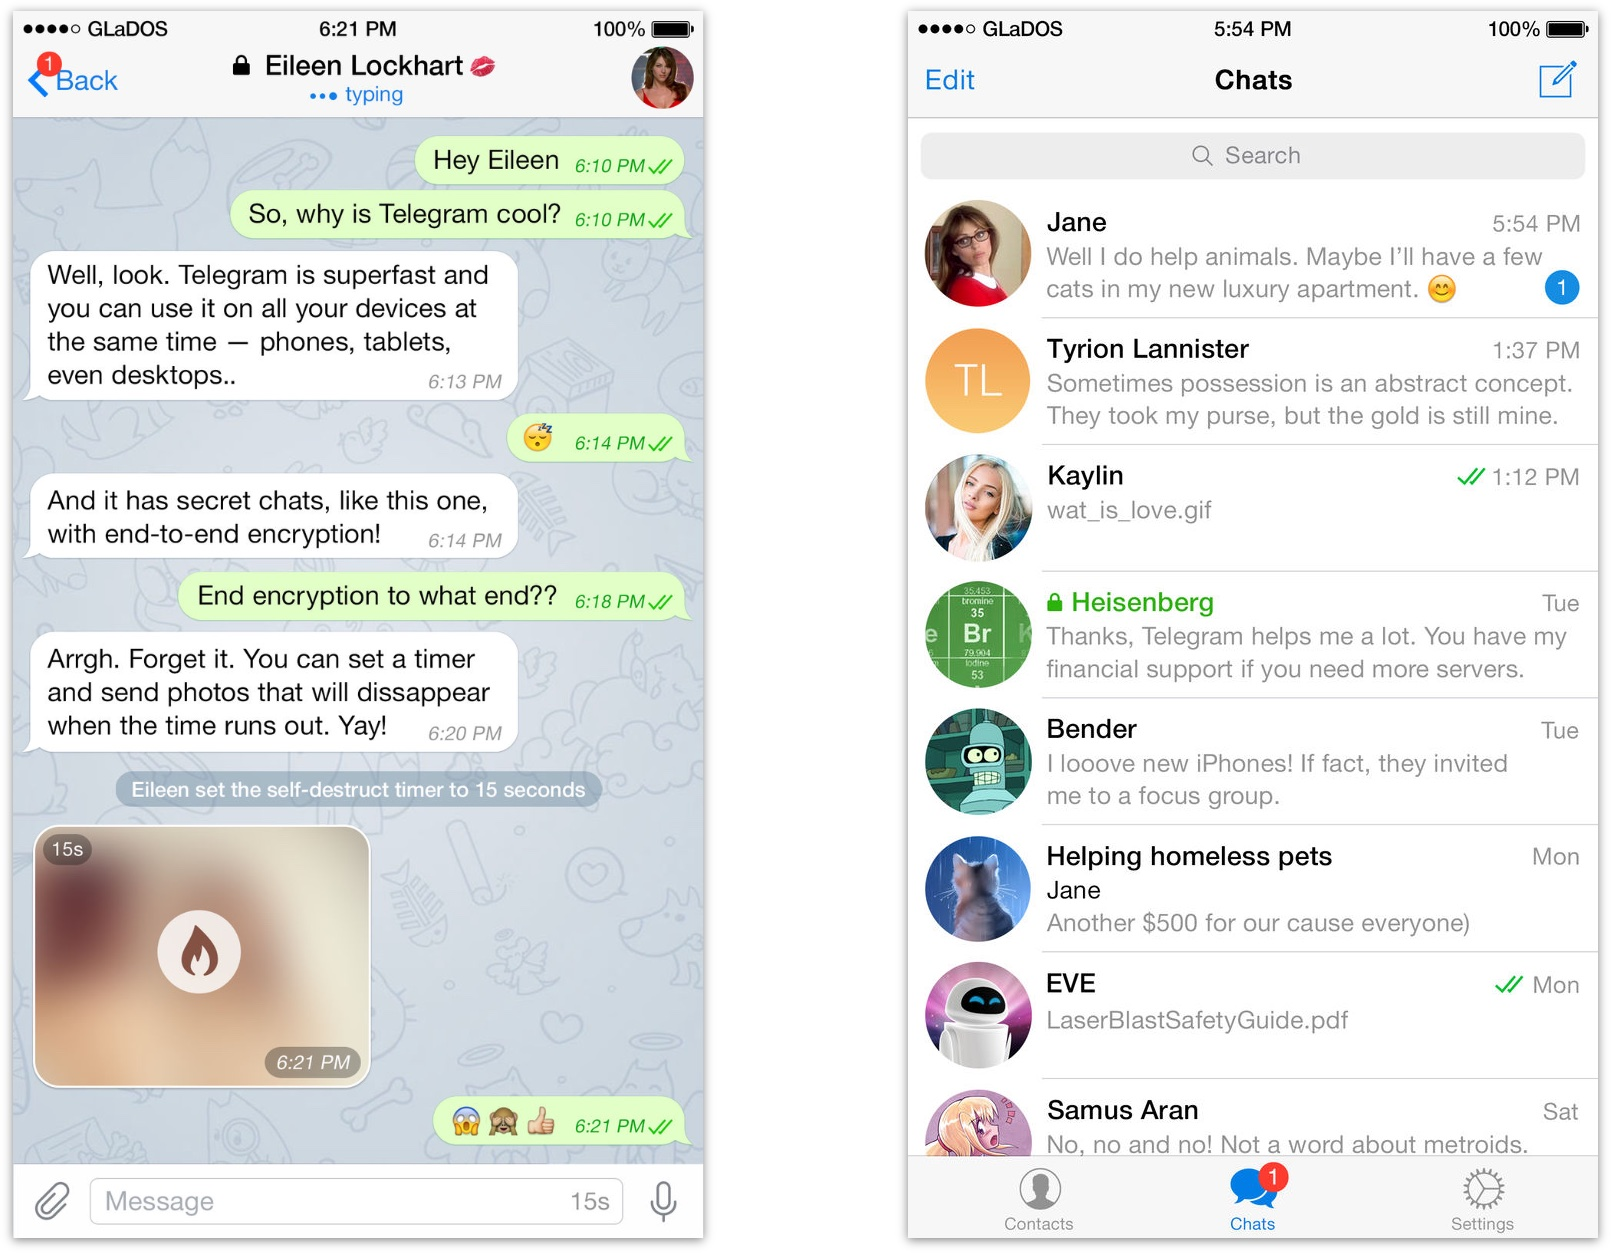
\includegraphics[width=0.75\textwidth]{inc/img/tg_combined.jpg}
  \caption{Дизайн клиента Telegram}
  \label{sec:analysis:research:analogs:telegram:ui}
\end{figure}

Стоит ближе рассмотреть протокол MTProto и~критику, направленую на~него. Протокол спроектирован для~доступа к серверному \gls{api} из~приложений, работающих на~мобильных устройствах. 
Протокол разделён на~три виртуально независимые части: 
\begin{itemize}
	\item \textbf{Высокоуровневый компонент (язык запросов)} -- определяет способ, посредством которого запросы и~ответы API преобразуются в~двоичные сообщения;
	\item \textbf{Уровень криптографии (авторизации)} -- определяет способ шифрования сообщений перед передачей через транспортный протокол;
	\item \textbf{Транспортный компонент} -- определяет метод для~клиента и~сервера для~передачи сообщений по~другому существующему сетевому протоколу (например, \gls{http}, \textit{HTTPS}, \textit{TCP}, \textit{UDP}).
\end{itemize}

На рисунке \ref{sec:analysis:research:analogs:telegram:mtproto1} представлена упрощённая схема взаимодействия клиента и~сервера, использующих протокол MTProto.

\begin{figure}[h]
  \centering
    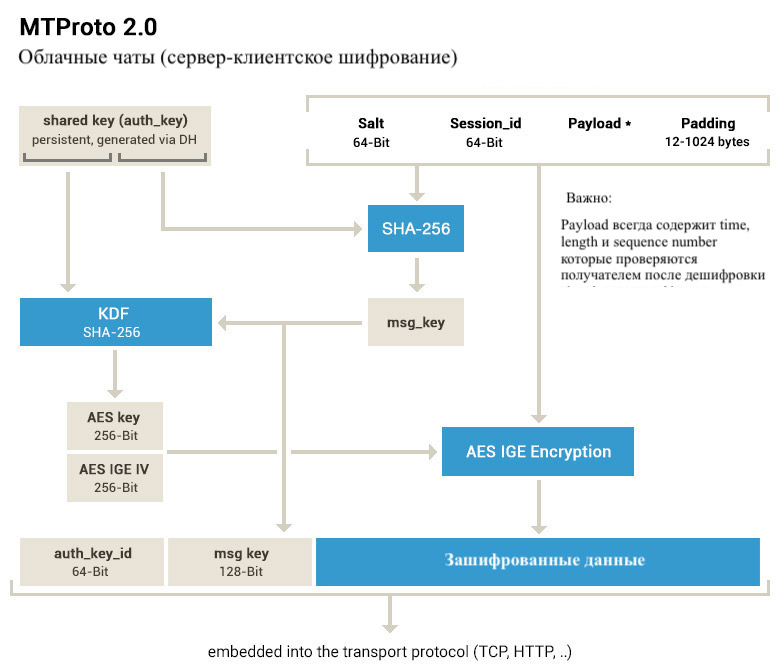
\includegraphics[width=0.8\textwidth]{inc/img/mtproto1.jpeg}
  \caption{Схема общения при помощи MTProto}
  \label{sec:analysis:research:analogs:telegram:mtproto1}
\end{figure}

Перед отправкой сообщения, оно зашифровывается определенным образом, а~над~ним добавляется \textit{внешний заголовок}, который представляет собой: 64-битный идентификатор ключа (который однозначно идентифицирует ключ авторизации для~сервера, а~также пользователя) и~128-битный ключ сообщения. Пользовательский ключ вместе с~ключом сообщения определяет фактический 256-битный ключ, который шифрует сообщение с~использованием шифрования \gls{aes}\textit{-256}. Стоит обратить внимание, что начальная часть сообщения, которая должна быть зашифрована, содержит переменные данные (сеанс, идентификатор сообщения, порядковый номер, соль сервера), который, очевидно, влияет на~ключ сообщения (и, следовательно, на~ключ \gls{aes} и~iv). Ключ сообщения определяется как 128 средних бит SHA256 тела сообщения (включая сеанс, идентификатор сообщения и~так далее).

Мессенджер распространяется бесплатно, не поддерживает корпоративные аккаунты и~использует собственную облачную архитектуру. Клиентские приложения пишутся сторонними командами, что несколько снижает уверенность в~криптографической стойскости всего продукта. Основным нареканием в~сторону протокола от~криптографических экспертов является его закрытость. Хорошие алгоритмы и~протоколы шифрования строятся на~математических доказательствах невозможности подобрать ключ шифрования в~разумное время и~свободно открывают реализацию для~публики, позволяя сообществу убедиться в~надёжности подхода и~помочь найти изъяны имплементации.
\subsubsection{}
\label{sec:analysis:research:analogs:imessage}

\textit{iMessage} -- проприетарное программное обеспечение от компании Apple, которое поставялется с дистрибьютивами почти всего семества современных операционных систем Apple:
\begin{itemize}
	\item iOS;
	\item macOS;
	\item watchOS.
\end{itemize}

iMessage интегрирован в приложения Messages на iOS и macOS, идентификаторами пользователей являются их мобильные номера или почта, привязанные к Apple ID. На рисунке \ref{sec:analysis:research:analogs:imessage:design} продемонстрирован дизайн приложения. Приложение поддерживает групповые чаты, расширения, является бесплатным для всех(и доступно только для) пользователей ОС, перечисленных выше.

\begin{figure}[h]
  \centering
    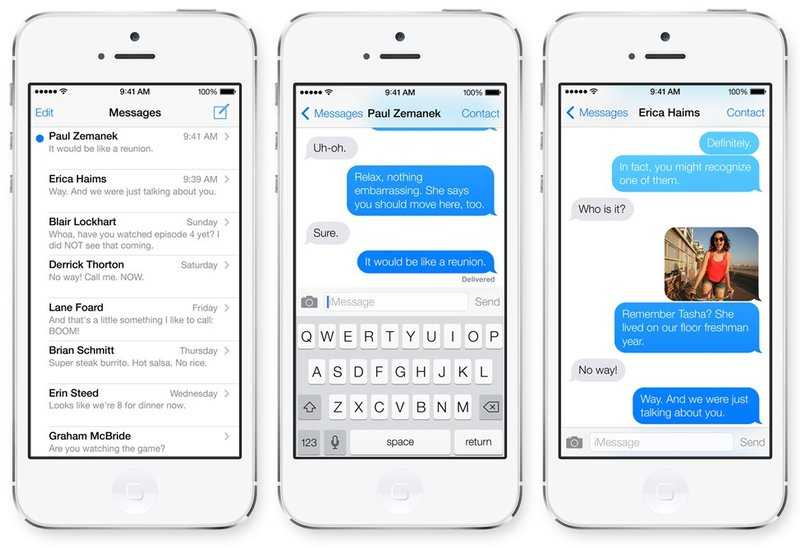
\includegraphics[width=0.75\textwidth]{inc/img/imdesign.jpeg}
  \caption{Дизайн iMessage}
  \label{sec:analysis:research:analogs:imessage:design}
\end{figure}

Коммуникационный протокол iMessage основан на Apple Push Notification Service -- прориетарном бинарном протоколе Apple. Телефон поддерживает постоянное соединение с серверами Apple, каждое соединение имеет собственный уникальный код, выступающий идентификатором. Соединение зашифровано при помощи TLS, используя сертификат устройства, который создаётся и отправляется на сервера Apple при активации утройства.
Криптографический протокол iMessage работает следующим образом:

\begin{enumerate}
	\item При активации iMessage на устройстве, генерируется две пары ассиметричных ключей: одна для шифрования и вторая для верификации.
	\item Публичные ключи отправляются на сервера Apple, а приватные никогда не покидают устройство.
	\item Когда кто-то начинает диалог, его устройство получает все публичные ключи участников диалога.
	\item При отправке сообщения, формируется \(n\) сообщений, каждое зашифрованно \(i\)-ым публичным ключом, где \(n\) -- количество устройств в диалоге.
\end{enumerate}

Недостатком данного подхода является потенциальная возможность Apple добавить собственный публичный ключ в список публичных ключей получателя, таким образом получив свою копию зашифрованного сообщения.

Как и было заявлено ранее, самые популярные конкуренты приложения выбрали путь закрытого программного обеспечения, отнимающего контроль у администраторов и бизнеса, что оправдывает разработку данного \gls{pp}.